\documentclass[10pt,times,twocolumn]{article}
\usepackage[normalem]{ulem}
%\usepackage{geometry}

%\pagestyle{plain}
\usepackage{caption}
\usepackage{times}
\usepackage{oneinchmargins}
\usepackage{tightenum}

\usepackage[toc,page]{appendix}

\usepackage{subfig}
\usepackage[normalem]{ulem}

%\usepackage{hyperref,url}%,bibunits}
\usepackage[hidelinks]{hyperref}
%\urlstyle{rm}
\usepackage[numbers,sort]{natbib}

%

\usepackage{setspace}
%\usepackage{epsf}
\usepackage{epsfig}
\usepackage{graphicx}
\usepackage{times}
%\usepackage{algorithm}
%\usepackage{algorithmic}
\usepackage{amsmath}
\usepackage[compact]{titlesec}
\usepackage{url}
%\usepackage{nonfloat}
\urlstyle{rm}
%\usepackage{algorithmic}
% \titlespacing*{\section}{0em}{-0ex}{-2ex}
% \titlespacing*{\subsection}{0em}{-0ex}{-2ex}
% \titlespacing*{\subsubsection}{0em}{-0ex}{-2ex}
%\setstretch{0.98}

\usepackage{multirow}


\usepackage{tikz}
\usetikzlibrary{calc}
\newcommand*\circled[1]{\tikz[baseline=-3pt]{
            \node[shape=circle,draw,inner sep=1pt,minimum size=10pt] (char) {\small #1};}}

%\setstretch{2.2}
%\setlength{\textheight}{9in}
%\setlength{\textwidth}{6.4in}
%\setlength{\oddsidemargin}{0in}
%\setlength{\evensidemargin}{0in}
%\setlength{\topmargin}{1in}
\usepackage{geometry}
%\geometry{lmargin=0.75in,rmargin=0.75in,tmargin=1in,bmargin=1in}
\geometry{reset, letterpaper, height=9in, width=7in, hmarginratio=1:1, vmarginratio=1:1, marginparsep=0pt, marginparwidth=0pt, headheight=15pt}

%\setlength{\textheight}{9.0in}
%\setlength{\columnsep}{0.33in}
%\setlength{\textwidth}{7.00in}
%\setlength{\topmargin}{0.0in}
%\setlength{\headheight}{0.0in}
%\setlength{\headsep}{0.0in}
%\addtolength{\oddsidemargin}{-0.25in}
%\addtolength{\evensidemargin}{-0.25in}
%\usepackage{usenix2019_v3}


  \let\oldthebibliography=\thebibliography
  \let\endoldthebibliography=\endthebibliography
  \renewenvironment{thebibliography}[1]{%
    \begin{oldthebibliography}{#1}%
      \setlength{\parskip}{0ex}%
      \setlength{\itemsep}{0ex}%
  }%
  {%
    \end{oldthebibliography}%
  }

%\setlength{\rightmargin}{0.0in}
%\setlength{\topmargin}{-0.5in}
%\setlength{\textheight}{9.6in}
%\setlength{\textwidth}{7.0in}
%\setlength{\oddsidemargin}{-0.275in}
%\setlength{\evensidemargin}{-0.275in}

%\newcommand{\ignore}[1]{}
%\setlength{\rightmargin}{-0.3in}
%\setlength{\topmargin}{-0.6in}
%\setlength{\textheight}{9.8in}
%\setlength{\textwidth}{7.5in}
%\setlength{\oddsidemargin}{-0.55in}
%\setlength{\evensidemargin}{-0.55in}

%\setlength{\topmargin}{-0.5in}
%\setlength{\textheight}{9.2in}
%\setlength{\textwidth}{6.9in}
%\setlength{\oddsidemargin}{-0.25in}
%\setlength{\evensidemargin}{-0.25in}



\usepackage{listings}
  \usepackage{courier}
 \lstset{
         basicstyle=\footnotesize\ttfamily, % Standardschrift
         %numbers=left,               % Ort der Zeilennummern
         numberstyle=\tiny,          % Stil der Zeilennummern
         %stepnumber=2,               % Abstand zwischen den Zeilennummern
         numbersep=5pt,              % Abstand der Nummern zum Text
         tabsize=2,                  % Groesse von Tabs
         extendedchars=true,         %
         breaklines=true,            % Zeilen werden Umgebrochen
         keywordstyle=\color{red},
    		frame=b,         
 %        keywordstyle=[1]\textbf,    % Stil der Keywords
 %        keywordstyle=[2]\textbf,    %
 %        keywordstyle=[3]\textbf,    %
 %        keywordstyle=[4]\textbf,   \sqrt{\sqrt{}} %
         stringstyle=\color{white}\ttfamily, % Farbe der String
         showspaces=false,           % Leerzeichen anzeigen ?
         showtabs=false,             % Tabs anzeigen ?
         xleftmargin=17pt,
         framexleftmargin=17pt,
         framexrightmargin=5pt,
         framexbottommargin=4pt,
         %backgroundcolor=\color{lightgray},
         showstringspaces=false      % Leerzeichen in Strings anzeigen ?        
 }
 \lstloadlanguages{% Check Dokumentation for further languages ...
         %[Visual]Basic
         %Pascal
         C
         %C++
         %XML
         %HTML
         %Java
 }

\sloppy

\newcommand{\mycaption}[3]{\beforecaption\caption{\label{#1}{\bf #2} \em\small #3}\aftercaption}

\newcommand{\BigO}[1]{${\cal O}(#1)$}
\newcommand{\BigOmega}[1]{$\Omega(#1)$}
\newcommand{\BigTheta}[1]{$\Theta(#1)$}

% only foreign words should be italicized... (example given should not)
\newcommand{\eg}{\textit{e.g.}}
\newcommand{\ie}{\textit{i.e.}}
\newcommand{\etal}{\textit{et al.}}
\newcommand{\etc}{\textit{etc.}}
\newcommand{\adhoc}{\textit{ad hoc}}

% units
\newcommand{\KB}{\,KB}
\newcommand{\MB}{\,MB}
\newcommand{\GB}{\,GB}
\newcommand{\TB}{\,TB}
\newcommand{\MBs}{\,MB/s}
\newcommand{\KBs}{\,KB/s}
\newcommand{\Kbs}{\,Kbit/s}
\newcommand{\mbs}{\,Mbit/s}
\newcommand{\mus}{\mbox{\,$\mu s$}}
\newcommand{\ms}{\mbox{\,$ms$}}

\renewcommand{\em}{\it}
\newcommand{\x}{$\times$}

% lego
\newcommand{\splitkernel}{splitkernel}
\newcommand{\lego}{LegoOS}
\newcommand{\ib}{IB}
\newcommand{\ibverbs}{IB-Verbs}
\newcommand{\rdma}{RDMA}
\newcommand{\dcrack}{DC-Rack}
\newcommand{\vnode}{vNode}
\newcommand{\vip}{vIP}
\newcommand{\vmount}{vMount}
\newcommand{\mmap}{{\texttt{mmap}}}
\newcommand{\munmap}{{\texttt{munmap}}}
\newcommand{\mremap}{{\texttt{mremap}}}
\newcommand{\grm}{GRM}
\newcommand{\gmm}{GMM}
\newcommand{\gsm}{GSM}
\newcommand{\gpm}{GPM}
\newcommand{\excache}{ExCache}
\newcommand{\vicache}{VtmCache}
\newcommand{\vregion}{vRegion}
\newcommand{\microos}{monitor}
%\newcommand{\microos}{$\mu$OS}
\newcommand{\brk}{{\texttt{brk}}}
\newcommand{\pcomponent}{pComponent}
\newcommand{\mcomponent}{mComponent}
\newcommand{\scomponent}{sComponent}

% dsnvm
\newcommand{\dsnvm}{DSPM}
\newcommand{\dsm}{DSM}
\newcommand{\nvm}{PM}
\newcommand{\hotpot}{Hotpot}
\newcommand{\mrmw}{MRMW}
\newcommand{\mrsw}{MRSW}
\newcommand{\wfetch}{FETCH}
\newcommand{\cd}{CD}
\newcommand{\dr}{DR}
\newcommand{\on}{ON}
\newcommand{\dn}{DN}
\newcommand{\xn}{CN}
\newcommand{\master}{MN}
\newcommand{\xactid}{CID}
\newcommand{\dirty}{dirty}
\newcommand{\committed}{committed}
\newcommand{\redundant}{redundant}
\newcommand{\ib}{IB}
\newcommand{\sendreply}{\texttt{send-reply}}
\newcommand{\atomicsendreply}{\texttt{atomic-send-reply}}
\newcommand{\multisendreply}{\texttt{multicast-send-reply}}
\newcommand{\journaled}{JOURNALED}
\newcommand{\fsyncsafe}{FSYNC\_SAFE}
\newcommand{\X}{{$\times$}}
\newcommand{\pmfs}{PMFS}
\newcommand{\tmpfs}{tmpfs}
\newcommand{\Octopus}{Octopus}
\newcommand{\Mojim}{Mojim}
\newcommand{\dsmnoxact}{DSM-NoXact}
\newcommand{\dsmxact}{DSM-Xact}
\newcommand{\clflush}{\texttt{clflush}}
\newcommand{\pcommit}{\texttt{pcommit}}
\newcommand{\mfence}{\texttt{mfence}}
\newcommand{\sfence}{\texttt{sfence}}
\newcommand{\ra}{\textbf{R1.a}}
\newcommand{\rb}{\textbf{R1.b}}
\newcommand{\rcs}{\textbf{R2.a}}
\newcommand{\rcm}{\textbf{R2.b}}
\newcommand{\rdr}{\textbf{R3.r}}
\newcommand{\rdu}{\textbf{R3.u}}
\newcommand{\re}{\textbf{R3}}
\newcommand{\rf}{\textbf{R4}}

%\newcommand{\ignore}[1]{}
\newif\ifremark
\long\def\remark#1{
\ifremark%
        \begingroup%
        \dimen0=\columnwidth
        \advance\dimen0 by -1in%
        \setbox0=\hbox{\parbox[b]{\dimen0}{\protect\em #1}}
        \dimen1=\ht0\advance\dimen1 by 2pt%
        \dimen2=\dp0\advance\dimen2 by 2pt%
        \vskip 0.25pt%
        \hbox to \columnwidth{%
                \vrule height\dimen1 width 3pt depth\dimen2%
                \hss\copy0\hss%
                \vrule height\dimen1 width 3pt depth\dimen2%
        }%
        \endgroup%
\fi}

%% Leave this on, so we can see them!!!
\remarktrue
\newcommand{\shortenum}{\vspace*{-0.1in}}
%\newcommand{\shortsec}{\vspace*{-0.2in}}
%\newcommand{\sparagraph}[1]{\vspace*{-0.2in}\paragraph{#1}}
%\newcommand{\sparagraph}[1]{\vspace*{-0.15in}\paragraph{#1}}
\newcommand{\sparagraph}[1]{\vspace*{0.0in}\paragraph{#1}}

% add below for confidential distribution
%\usepackage{draftwatermark}
%\SetWatermarkText{DO NOT DISTRIBUTE}
%\SetWatermarkScale{0.4}


\pagestyle{plain}


%\input{summary}
%\clearpage
%\pagestyle{myheadings}
%\pagenumbering{arabic}

%\newenvironment{smallitemize}{\begin{list}{$\bullet$}{\topsep0.0in\itemsep0.0in\parsep0.0in\partopsep0.0in\itemindent0.1in\leftmargin0.1in}}{\end{list}}
%\newenvironment{smallitemize}{\begin{list}{$\bullet$}{\topsep0.1in\itemsep0.1in\parsep0.1in\partopsep0.1in\itemindent0.1in\leftmargin0.1in}}{\end{list}}
%\newenvironment{smallitemize}{\begin{list}{$\bullet$}{\topsep0.05in\itemsep0.05in\parsep0.0in\partopsep0.05in\itemindent0.05in\leftmargin0.05in}}{\end{list}}
%{\topsep{0in}\itemsep{0.1in}\itemindent{0.1in}}
%%%%%%%%%%%%%%%%%%%%%%%%



\newcommand{\mm}{mm$^2$}
\newcommand{\figtitle}[1]{\textbf{#1}}
\newcommand{\us}{$\mu$s}
\newcommand{\fixme}[1]{{\color{red}\textbf{#1}}}

\definecolor{pink}{rgb}{1.0,0.47,0.6}
\newcommand{\adrian}[1]{{\color{green}\textbf{#1}}}
\newcommand{\laura}[1]{{\color{pink}\textbf{#1}}}
\newcommand{\joel}[1]{{\color{red}\textbf{#1}}}
\newcommand{\ameen}[1]{{\color{blue}\textbf{#1}}}
\newcommand{\arup}[1]{{\color{yellow}\textbf{#1}}}
\newcommand{\hungwei}[1]{{\color{purple}\textbf{#1}}}


\newcommand{\note}[2]{\fixme{$\ll$ #1 $\gg$ #2}}

\newcommand{\myitem}[1]{\item \textbf{#1}}

\lstloadlanguages{% Check Dokumentation for further languages ...
        %[Visual]Basic
        %Pascal
        C
        %C++
        %XML
        %HTML
        %Java
}

\lstdefinestyle{customc}{
  belowcaptionskip=1\baselineskip,
  breaklines=true,
  frame=b,
  xleftmargin=\parindent,
  language=C,
  showstringspaces=false,
  basicstyle=\scriptsize\ttfamily,
  keywordstyle=\bfseries\color{green!40!black},
  commentstyle=\itshape\color{purple!40!black},
  identifierstyle=\color{blue},
  stringstyle=\color{red},
}
\lstset{escapechar=@,style=customc}


\begin{document}

\begin{appendices}

\section{\phdm\ Use Cases}
Many types of applications can make use of \phdm.
Below we give some examples. % on what services an \phdm\ system can provide and how applications can use them.
We implemented an instance of the first three types in this paper,
leaving the rest for future work.

\boldpara{Extended (semantic-rich) virtual memory.}
A basic service \phdm\ can provide is a remote virtual memory space that lets applications
store in-memory data (\eg, as extended, slower heaps).
In addition to simple, hardware-like virtual memory APIs such as reading and writing to a memory address, 
\phdm\ could provide higher-level APIs like synchronization primitives, pointer manipulation, 
vector and scatter-gather operations~\cite{Aguilera-FarMemory}.
Applications and language libraries can then build complex data structures like vectors 
and trees with these APIs.

\boldpara{In-memory and ephemeral storage.}
\phdm\ could offer in-memory storage services such as distributed key-value stores, databases, and file systems.
With \phdm, many storage operations (\eg, key-value pair lookup, SQL select) 
could be implemented in hardware at where the data is, offering enhanced performance. 
\phdm\ is also a good fit for building ephemeral storage and storage caching that do not require failure resilience~\cite{SnowFlake-NSDI20,Pocket,fitzpatrick2004distributed}.
%We implemented a distributed key-value store in \sys\ with optional replication support.

\boldpara{Data sharing.}
Since multiple \CN{}s can access the same \MN{}s in \phdm,
\phdm\ could be used for data sharing and communication across \CN{}s.
This is especially useful for new datacenter services like serverless computing~\cite{Berkeley-Serverless},
which currently has no or poor support for managing states and inter-function communication.
With \phdm, serverless functions can run on \CN{}s and store states or communication messages in the disaggregated memory layer.
Similarly, \phdm\ can also be used for storing global states such as the parameter server in distributed machine learning systems.
%We implemented a multi-version data sharing service in \sys\
%that can be accessed by different \CN{}s concurrently.

\boldpara{Offloading data processing.}
\phdm\ is a good candidate for offloading data processing and data analytics. 
Data-intensive applications can offload computation that frequently access in-memory data together with 
these data to \MN{}s.
One such example is disaggregated Spark shuffle~\cite{Stuedi-ATC19}, where the shuffle
operation could be implemented in programmable hardware and the shuffle data could be 
stored in \MN{}s of \phdm.

\boldpara{Remote swap and remote disk.}
Legacy applications and libraries can also benefit from \phdm\ in a transparent way.
Two such examples are remote memory-based disk and remote swap~\cite{InfiniSwap}.
The OS at the \CN{}s can add a memory-based block device that sits in \phdm\
in a similar way as building the {\em ramdisk} module.
Applications can directly use this new device or use it as a swap space.

\boldpara{Disaggregated OS.}
Recently, there have been proposals to completely disaggregate memory from compute.
\lego~\cite{Shan18-OSDI} is such a proposal that organizes compute nodes as processors with no memory 
and \MN{}s as memory devices with no computation.
\lego\ can build on \phdm\ by configuring \CN{}s as its compute nodes %(called {\em pComponent}s) 
and \MN{}s as its memory nodes. %(called {\em mComponent}s).

\section{Discussion}
\label{sec:discussion}

\ulinebfpara{Hardware choice.}
A key contribution of \sys\ is our demonstration of how to best separate 
data and metadata planes into hardware and software components.
This conceptual separation could be adopted by future system builders
in addition to our specific implementation of \sys.
%We intentionally separate out this conceptual demonstration from a 
Although we developed \sys's hardware components all on a single FPGA,
we do not see it as the only way to build the hardware part of \sys.
Another promising approach is to separate out the fixed logics in \sys\ hardware components
into an ASIC and the rest in FPGA. 
For example, for environments that do not need customization of network or the core-memory stack,
they could be integrated into one ASIC based network controller to provide fast network/memory accesses,
ASIC based memory controller IPs can also be added to provide modern CPU level memory access performance.
while extended services are still deployed on an FPGA.
%The ASIC and the FPGA could be integrated into the same die or same chip for faster communication.
Note that this ASIC would still be very different from today's RDMA NIC,
as our stacks have a client-centric addressing view.
Also note that there are still cases where users would want to customize \sys's network and the core-memory stack,
\eg, to provide better performance isolation and security.


%\ulinebfpara{Data caching.}

\ulinebfpara{Security and performance isolation.}
\sys\ currently adopts traditional address-space-based protection mechanisms to 
isolate application processes from each other 
and to restrict non-\sys\ owners from changing \sys\ or other user's hardware and software.
When deployed in the cloud, multi-tenancy environment that requires stronger security and/or performance isolation (\eg, to prevent side-channel attacks),
and our current implementation of \sys\ needs some adaptation. % to provide stronger security and performance isolation.
For example, the PTE cache currently is shared across application processes,
and there is no network bandwidth limits for an individual connection.
It is fairly easy to change them to provide more isolation and SLA guarantees,
and we leave it for future work. % isolation between processes.

\ulinebfpara{Failure handling.}
Although memory systems are usually assumed to be volatile, % (\ie, in-memory data can be lost),
there are still situations that require proper failure handling (\eg, for high availability or to use memory for storage data).
As there can be many ways to build memory services on \sys\ 
and many such services are already or would benefit from handling failure on their own,
we believe that there should not be any built-in failure handling mechanism in \sys.
Instead, \sys\ should offer primitives like replicated writes for users to build their own services.
We leave adding such API extensions to \sys\ as future work.
%The usage of \sys\ ranges from temporarily hosting cached or ephemeral data to permanently storing data.

\ulinebfpara{Client-side.}
An interesting finding we have is that client-side systems
could become a performance bottleneck after we made the remote memory layer very fast.
Surprisingly, most of our performance tuning efforts are spent on the client side (\eg, thread model, network stack implementation).
More future research could go into finding the best way for client applications to fully exploit \sys's remote memory performance.


% {
% \begin{figure}[h]
% \begin{minipage}[t]{0.47\columnwidth}
% \begin{center}
% \centerline{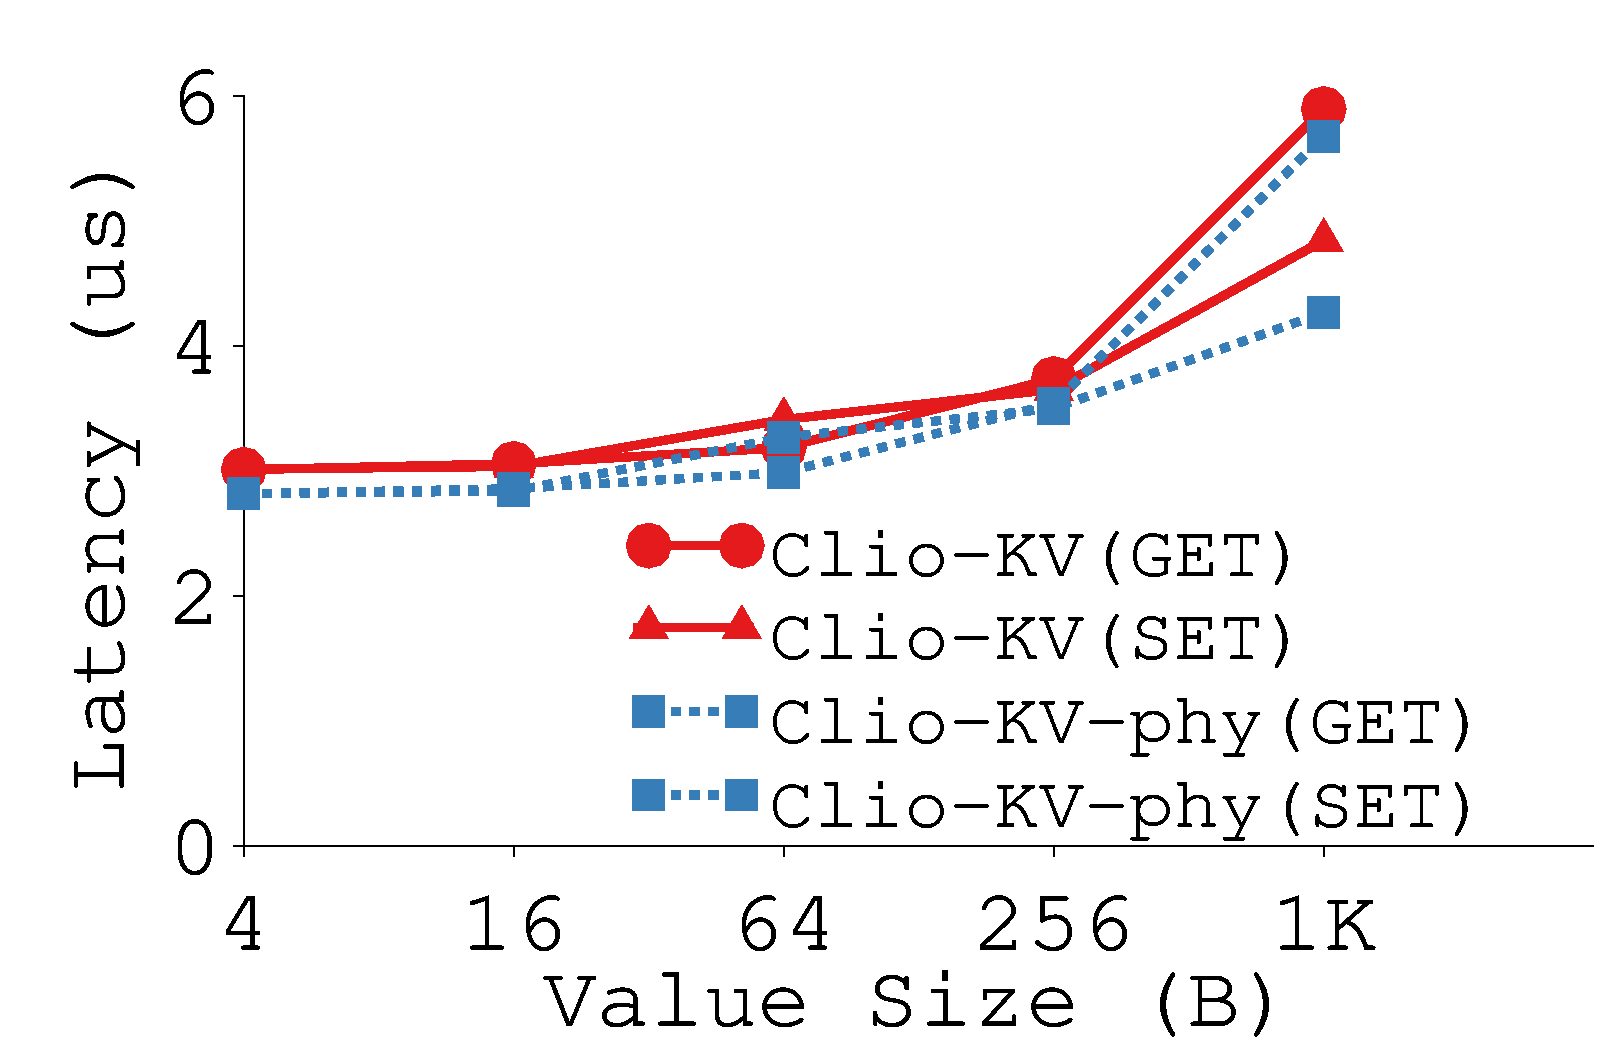
\includegraphics[width=\columnwidth]{Figures/g_plot_kvs_latency.pdf}}
% \mycaption{fig-kvs-latency}{GET/SET Latency.}
% {
% With one \MN\ and one 1\CN, vary by request size.
% }
% \end{center}
% \end{minipage}
% \hfill
% \begin{minipage}[t]{0.47\columnwidth}
% \begin{center}
% \centerline{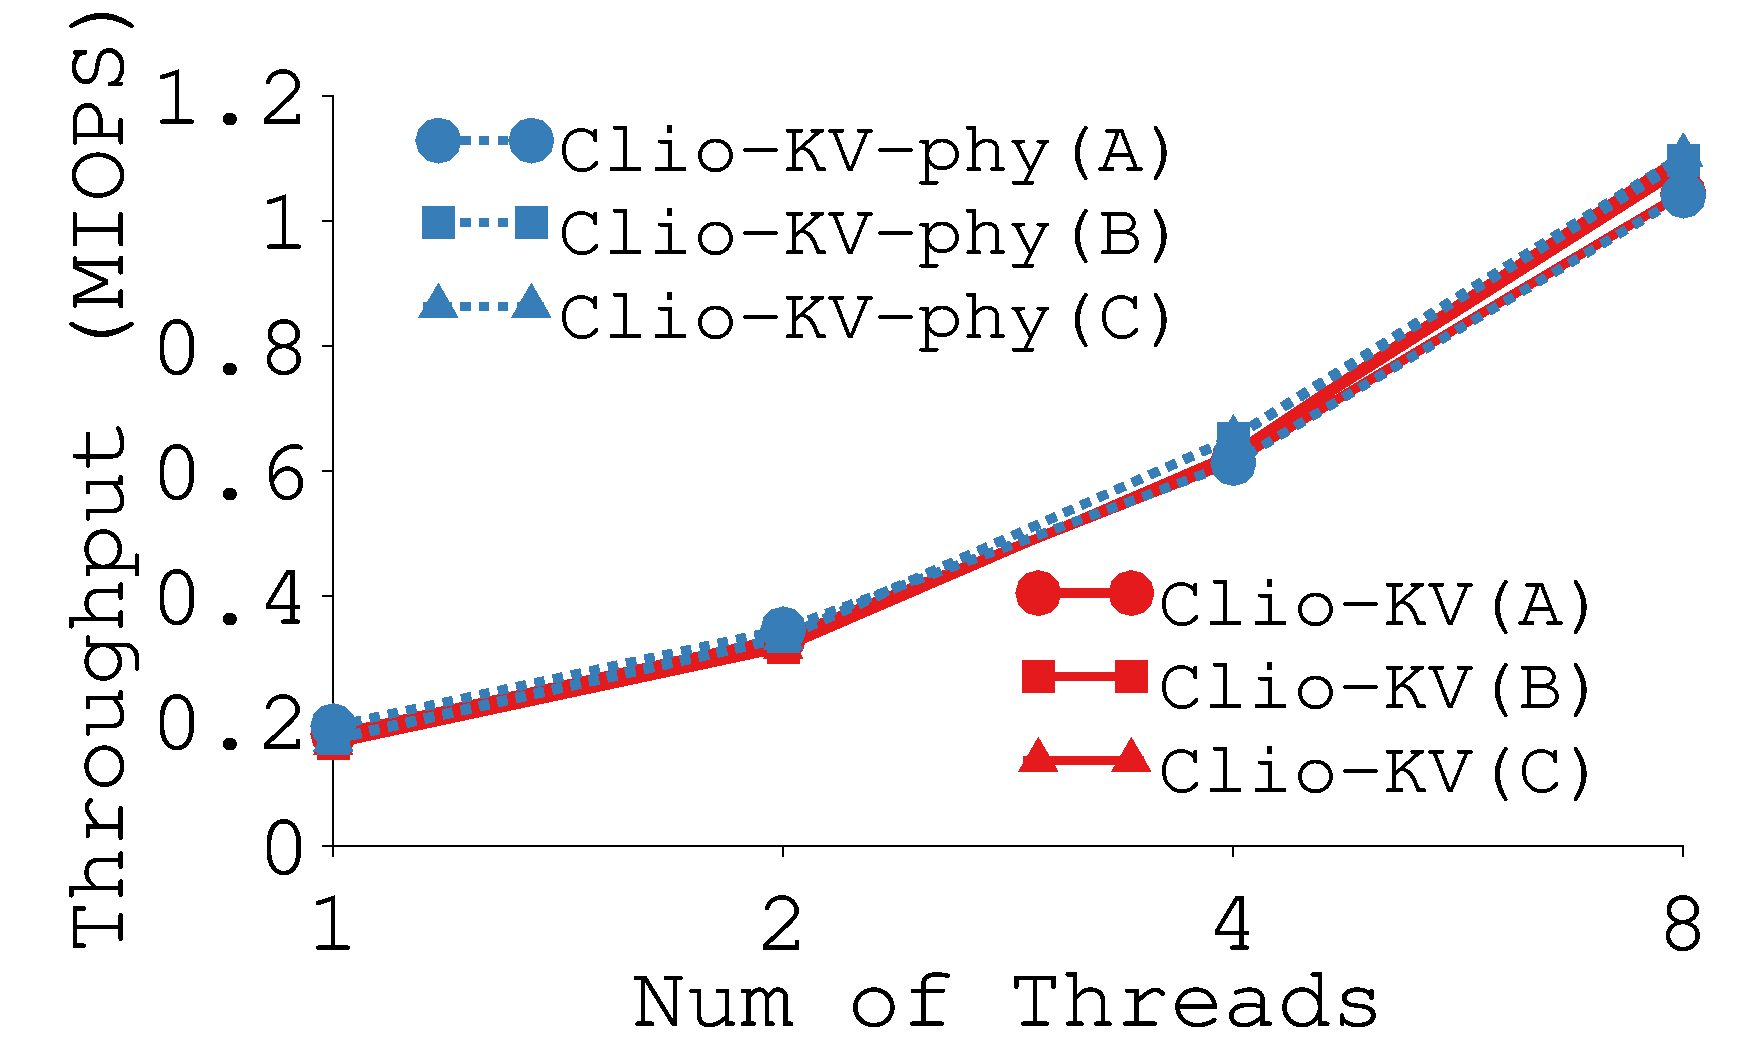
\includegraphics[width=\columnwidth]{Figures/g_plot_ycsb_thread.pdf}}
% \mycaption{fig-kvs-tput}{YCSB Throughput.}
% {
% With one \MN\ and one 1\CN, vary by number of threads.
% }
% \end{center}
% \end{minipage}
% \end{figure}
% }

% \section{Key-Value Stores on Clio}
% To compare with \syskv\ and to demonstrate different ways of implementing extended services, 
% we implemented a key-value store with the same design but directly uses raw physical memory.
% We call it {\em \syskvphys}.
% %From our experiments, \syskv\ adds 4\%--13\% latency overhead and 1\%--5\% throughput overhead over this raw key-value store implementation (see Appendix for detailed results).
% Figure~\ref{fig-kvs-latency} and Figure~\ref{fig-kvs-tput} show the latency and throughput comparison.
% Both systems achieve low latency similar to \sys's read/write performance.
% \syskv\ adds 4\%--13\% latency overhead and 1\%--5\% throughput overhead over \syskvphys.
% %Building extended services on \sys's virtual memory interface is easier and incurs reasonable performance overhead.
% %But for services that desire optimal performance, it is best to build them on \sys's platform but with direct physical memory accesses. %anot only easier but also largely preserves low-level performance.

\section{\sys\ Address Translation}

Figure~\ref{fig-coremem-diagram} shows the detailed state diagram of \sys's FPGA
core-memory module.
%Following figure shows Clio \MN{} internal FPGA state diagram.

{
\begin{figure}[!ht]
\begin{minipage}{\columnwidth}
\begin{center}
\centerline{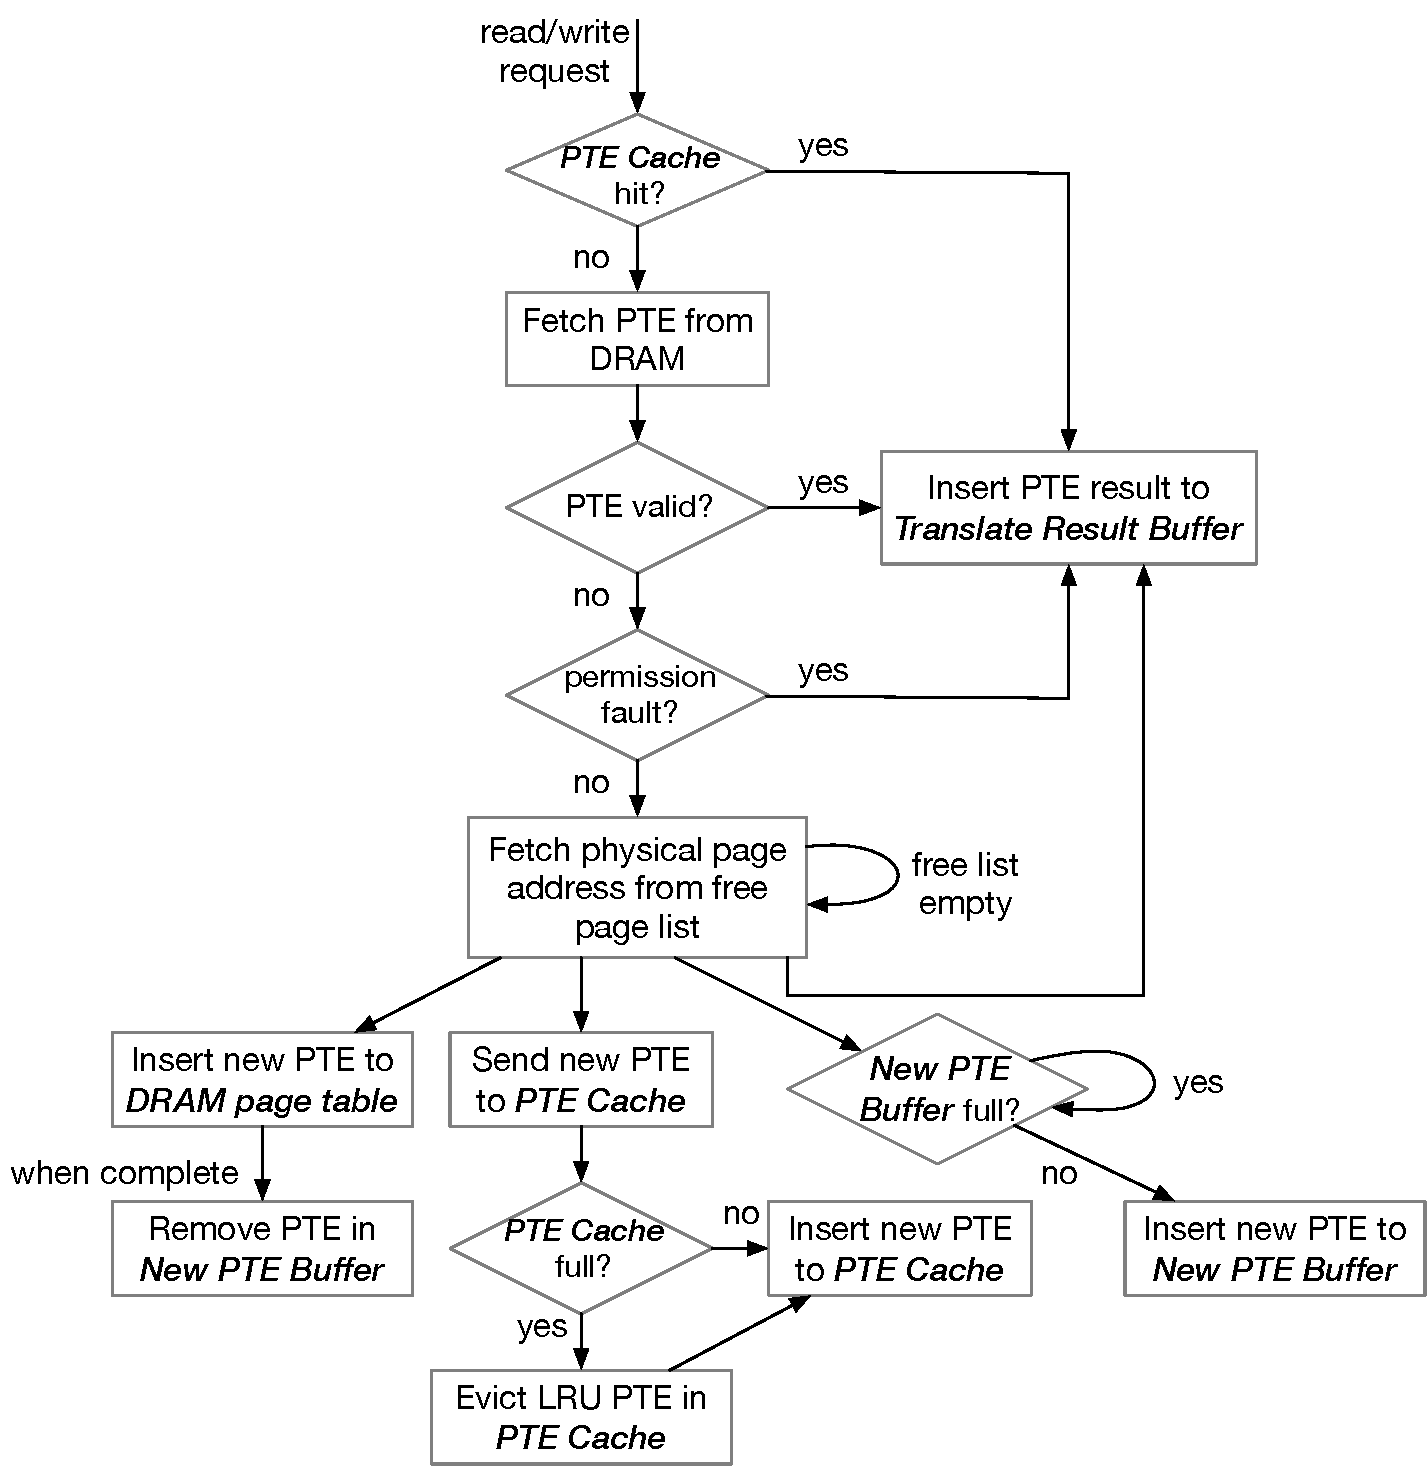
\includegraphics[width=\textwidth]{Figures/CoreMemStateDiagram.pdf}}
\mycaption{fig-coremem-diagram}{Core-Memory Address Translation State Diagram.}
{
}
\end{center}
\end{minipage}
\end{figure}
}

\end{appendices}

%\clearpage
\bibliographystyle{plain}
\bibliography{all-defs,all,personal,all-confs,local,paper}
\end{document}
